%% (Master) Thesis template
% Template version used: v1.4
%
% Largely adapted from Adrian Nievergelt's template for the ADPS
% (lecture notes) project.


%% We use the memoir class because it offers a many easy to use features.
\documentclass[11pt,a4paper,titlepage]{memoir}

%% Packages
%% ========

%% LaTeX Font encoding -- DO NOT CHANGE
\usepackage[OT1]{fontenc}

%% Babel provides support for languages.  'english' uses British
%% English hyphenation and text snippets like "Figure" and
%% "Theorem". Use the option 'ngerman' if your document is in German.
%% Use 'american' for American English.  Note that if you change this,
%% the next LaTeX run may show spurious errors.  Simply run it again.
%% If they persist, remove the .aux file and try again.
\usepackage[english]{babel}

%% Input encoding 'utf8'. In some cases you might need 'utf8x' for
%% extra symbols. Not all editors, especially on Windows, are UTF-8
%% capable, so you may want to use 'latin1' instead.
\usepackage[utf8]{inputenc}

%% This changes default fonts for both text and math mode to use Herman Zapfs
%% excellent Palatino font.  Do not change this.
\usepackage[sc]{mathpazo}

%% The AMS-LaTeX extensions for mathematical typesetting.  Do not
%% remove.
\usepackage{amsmath,amssymb,amsfonts,mathrsfs}
\usepackage{bm}

%% NTheorem is a reimplementation of the AMS Theorem package. This
%% will allow us to typeset theorems like examples, proofs and
%% similar.  Do not remove.
%% NOTE: Must be loaded AFTER amsmath, or the \qed placement will
%% break
\usepackage[amsmath,thmmarks]{ntheorem}

%% LaTeX' own graphics handling
\usepackage{graphicx}

%% We unfortunately need this for the Rules chapter.  Remove it
%% afterwards; or at least NEVER use its underlining features.
\usepackage{soul}

%% This allows you to add .pdf files. It is used to add the
%% declaration of originality.
\usepackage{pdfpages}

%% Some more packages that you may want to use.  Have a look at the
%% file, and consult the package docs for each.
%% See the TeXed file for more explanations

%% [OPT] Multi-rowed cells in tabulars
%\usepackage{multirow}

%% [REC] Intelligent cross reference package. This allows for nice
%% combined references that include the reference and a hint to where
%% to look for it.
\usepackage{varioref}

%% [OPT] Easily changeable quotes with \enquote{Text}
%\usepackage[german=swiss]{csquotes}

%% [REC] Format dates and time depending on locale
\usepackage{datetime}

%% [OPT] Provides a \cancel{} command to stroke through mathematics.
%\usepackage{cancel}

%% [NEED] This allows for additional typesetting tools in mathmode.
%% See its excellent documentation.
\usepackage{mathtools}

%% [ADV] Conditional commands
%\usepackage{ifthen}

%% [OPT] Manual large braces or other delimiters.
%\usepackage{bigdelim, bigstrut}

%% [REC] Alternate vector arrows. Use the command \vv{} to get scaled
%% vector arrows.
\usepackage[h]{esvect}

%% [NEED] Some extensions to tabulars and array environments.
\usepackage{array}

%% [OPT] Postscript support via pstricks graphics package. Very
%% diverse applications.
%\usepackage{pstricks,pst-all}

%% [?] This seems to allow us to define some additional counters.
%\usepackage{etex}

%% [ADV] XY-Pic to typeset some matrix-style graphics
%\usepackage[all]{xy}

%% [OPT] This is needed to generate an index at the end of the
%% document.
%\usepackage{makeidx}

%% [OPT] Fancy package for source code listings.  The template text
%% needs it for some LaTeX snippets; remove/adapt the \lstset when you
%% remove the template content.
\usepackage{listings}
\lstset{language=TeX,basicstyle={\normalfont\ttfamily}}

%% [REC] Fancy character protrusion.  Must be loaded after all fonts.
\usepackage[activate]{pdfcprot}

%% [REC] Nicer tables.  Read the excellent documentation.
\usepackage{booktabs}


%% Our layout configuration.  DO NOT CHANGE.
%% Memoir layout setup

%% NOTE: You are strongly advised not to change any of them unless you
%% know what you are doing.  These settings strongly interact in the
%% final look of the document.

% Dependencies
\usepackage{ETHlogo}

% Turn extra space before chapter headings off.
\setlength{\beforechapskip}{0pt}

\nonzeroparskip
\parindent=0pt
\defaultlists

% Chapter style redefinition
\makeatletter

\if@twoside
  \pagestyle{Ruled}
  \copypagestyle{chapter}{Ruled}
\else
  \pagestyle{ruled}
  \copypagestyle{chapter}{ruled}
\fi
\makeoddhead{chapter}{}{}{}
\makeevenhead{chapter}{}{}{}
\makeheadrule{chapter}{\textwidth}{0pt}
\copypagestyle{abstract}{empty}

\makechapterstyle{bianchimod}{%
  \chapterstyle{default}
  \renewcommand*{\chapnamefont}{\normalfont\Large\sffamily}
  \renewcommand*{\chapnumfont}{\normalfont\Large\sffamily}
  \renewcommand*{\printchaptername}{%
    \chapnamefont\centering\@chapapp}
  \renewcommand*{\printchapternum}{\chapnumfont {\thechapter}}
  \renewcommand*{\chaptitlefont}{\normalfont\huge\sffamily}
  \renewcommand*{\printchaptertitle}[1]{%
    \hrule\vskip\onelineskip \centering \chaptitlefont\textbf{\vphantom{gyM}##1}\par}
  \renewcommand*{\afterchaptertitle}{\vskip\onelineskip \hrule\vskip
    \afterchapskip}
  \renewcommand*{\printchapternonum}{%
    \vphantom{\chapnumfont {9}}\afterchapternum}}

% Use the newly defined style
\chapterstyle{bianchimod}

\setsecheadstyle{\Large\bfseries\sffamily}
\setsubsecheadstyle{\large\bfseries\sffamily}
\setsubsubsecheadstyle{\bfseries\sffamily}
\setparaheadstyle{\normalsize\bfseries\sffamily}
\setsubparaheadstyle{\normalsize\itshape\sffamily}
\setsubparaindent{0pt}

% Set captions to a more separated style for clearness
\captionnamefont{\sffamily\bfseries\footnotesize}
\captiontitlefont{\sffamily\footnotesize}
\setlength{\intextsep}{16pt}
\setlength{\belowcaptionskip}{1pt}

% Set section and TOC numbering depth to subsection
\setsecnumdepth{subsection}
\settocdepth{subsection}

%% Titlepage adjustments
\pretitle{\vspace{0pt plus 0.7fill}\begin{center}\HUGE\sffamily\bfseries}
\posttitle{\end{center}\par}
\preauthor{\par\begin{center}\let\and\\\Large\sffamily}
\postauthor{\end{center}}
\predate{\par\begin{center}\Large\sffamily}
\postdate{\end{center}}

\def\@advisors{}
\newcommand{\advisors}[1]{\def\@advisors{#1}}
\def\@department{}
\newcommand{\department}[1]{\def\@department{#1}}
\def\@thesistype{}
\newcommand{\thesistype}[1]{\def\@thesistype{#1}}

\renewcommand{\maketitlehooka}{\noindent\ETHlogo[2in]}

\renewcommand{\maketitlehookb}{\vspace{1in}%
  \par\begin{center}\Large\sffamily\@thesistype\end{center}}

\renewcommand{\maketitlehookd}{%
  \vfill\par
  \begin{flushright}
    \sffamily
    \@advisors\par
    \@department, ETH Z\"urich
  \end{flushright}
}

\checkandfixthelayout

\setlength{\droptitle}{-48pt}

\makeatother

% This defines how theorems should look. Best leave as is.
\theoremstyle{plain}
\setlength\theorempostskipamount{0pt}

%%% Local Variables:
%%% mode: latex
%%% TeX-master: "thesis"
%%% End:


%% Theorem environments.  You will have to adapt this for a German
%% thesis.
%% Theorem-like environments

%% This can be changed according to language. You can comment out the ones you
%% don't need.

\numberwithin{equation}{chapter}

%% German theorems
%\newtheorem{satz}{Satz}[chapter]
%\newtheorem{beispiel}[satz]{Beispiel}
%\newtheorem{bemerkung}[satz]{Bemerkung}
%\newtheorem{korrolar}[satz]{Korrolar}
%\newtheorem{definition}[satz]{Definition}
%\newtheorem{lemma}[satz]{Lemma}
%\newtheorem{proposition}[satz]{Proposition}

%% English variants
\newtheorem{theorem}{Theorem}[chapter]
\newtheorem{example}[theorem]{Example}
\newtheorem{remark}[theorem]{Remark}
\newtheorem{corollary}[theorem]{Corollary}
\newtheorem{definition}[theorem]{Definition}
\newtheorem{lemma}[theorem]{Lemma}
\newtheorem{proposition}[theorem]{Proposition}

%% Proof environment with a small square as a "qed" symbol
\theoremstyle{nonumberplain}
\theorembodyfont{\normalfont}
\theoremsymbol{\ensuremath{\square}}
\newtheorem{proof}{Proof}
%\newtheorem{beweis}{Beweis}


%% Helpful macros.
%% Custom commands
%% ===============

%% Special characters for number sets, e.g. real or complex numbers.
\newcommand{\C}{\mathbb{C}}
\newcommand{\K}{\mathbb{K}}
\newcommand{\N}{\mathbb{N}}
\newcommand{\Q}{\mathbb{Q}}
\newcommand{\R}{\mathbb{R}}
\newcommand{\Z}{\mathbb{Z}}
\newcommand{\X}{\mathbb{X}}

%% Fixed/scaling delimiter examples (see mathtools documentation)
\DeclarePairedDelimiter\abs{\lvert}{\rvert}
\DeclarePairedDelimiter\norm{\lVert}{\rVert}

%% Use the alternative epsilon per default and define the old one as \oldepsilon
\let\oldepsilon\epsilon
\renewcommand{\epsilon}{\ensuremath\varepsilon}

%% Also set the alternate phi as default.
\let\oldphi\phi
\renewcommand{\phi}{\ensuremath{\varphi}}


%% Make document internal hyperlinks wherever possible. (TOC, references)
%% This MUST be loaded after varioref, which is loaded in 'extrapackages'
%% above.  We just load it last to be safe.
\usepackage[linkcolor=black,colorlinks=true,citecolor=black,filecolor=black]{hyperref}


%% Document information
%% ====================

\title{Well-balanced methods for computation of the standing accretion shock instability (SASI)}
\author{Samuel Maloney}
\thesistype{Master Thesis}
\advisors{Advisors: Prof.\ Dr.\ Siddhartha Mishra, Dr.\ Roger Käppeli}
\department{Department of Mathematics, Seminar for Applied Mathematics}
\date{December 31, 2018}

\begin{document}

\frontmatter

%% Title page is autogenerated from document information above.  DO
%% NOT CHANGE.
\begin{titlingpage}
  \calccentering{\unitlength}
  \begin{adjustwidth*}{\unitlength-24pt}{-\unitlength-24pt}
    \maketitle
  \end{adjustwidth*}
\end{titlingpage}

%% The abstract of your thesis.  Edit the file as needed.
\begin{abstract}
  Simulating the standing accretion shock instability.
\end{abstract}


%% TOC with the proper setup, do not change.
\cleartorecto
\tableofcontents
\mainmatter

%% Your real content!
% Some commands used in this file
\newcommand{\package}{\emph}

\chapter{Introduction}

In the study of astrophysical entities, accretion shocks are a fairly commonly encountered physical phenomena. In particular, standing accretion shocks (SAS) are part of the theory behind core-collapse supernovae, with an instability (SASI) described by Blondin et al.~\cite{Blondin2003} being proposed as a possible mechanism for driving the explosive evolution of these phsyical systems. This instability occurs because of the spherical nature of the system, with the effects of perturbations to the symmetry of the shock being trapped in the interior subsonic region and producing feedback loops which further perturb the shock front.

To gain a better understanding of the underlying mechanisms of this instability, Foglizzo~\cite{Foglizzo2009} and Sato et al.~\cite{Sato2009} (hereafter referred to together as FS) proposed and studied a simple toy problem, the details of which are presented in Section \ref{sec:toyProblem}. Using this simple set-up they showed evidence for a coupled advective-acoustic cycle between the stationary shock front and an interior decelerating potential step that is intended to model the effects of matter settling onto the surface of the accreting object.

For this thesis, well-balanced methods for simulating steady states in the presence of external potential fields, as developed by K\"appeli and Mishra~\cite{Kappeli2014} (hereafter referred to as KM), were applied to the aforementioned toy problem as well as 2D simulations of the SASI scenario using circular and spherical geometries. The mathematical theory of fluid flow and associated steady states is briefly outlined in Section~\ref{sec:euler} while an overview of the numerical method and well-balanced scheme used for this thesis is given in Section~\ref{sec:numerics}.


\section{Euler Equations}
\label{sec:euler}

The time evolution of the dynamics of fluids can be described by systems of balance laws. For inviscid fluids, this system is given by the well-known Euler equations with source terms, which mathematically represent the physical conservation of mass, momentum, and energy. They are given here following the notation of KM as
\begin{subequations} \label{eq:eulerFull}
\begin{align}
\frac{\partial{\rho}}{\partial{t}} &+ \nabla \cdot (\rho \mathbf{v}) = 0,\\
\frac{\partial{\rho \mathbf{v}}}{\partial{t}} &+ \nabla \cdot (\mathbf{v} \rho \mathbf{v}) + \nabla p = -\rho \nabla \phi,\\
\frac{\partial{E}}{\partial{t}} &+ \nabla \cdot \left[(E+p)\mathbf{v}\right] = -\rho \mathbf{v} \cdot \nabla \phi,
\end{align}
\end{subequations}
where $\rho$ is the mass density, and $\mathbf{v}$ is the local velocity vector. $E$ is the total energy sum of the internal and kinetic energies given as
\begin{equation}
E=\rho e + \frac{\rho \mathrm{v}^2}{2}.
\end{equation}
An equation of state $p=p(\rho,e)$ must be selected for a given problem to complete the relations between these primitive quanitites. The quantitiy $\phi$ on the right-hand side of the latter two equations represents an external potential field (e.g.\ gravity) which acts upon the fluid. For our purposes, this potential is assumed to be known, either as a given value, through pre-computation, or by solving for it independently of the other fluid quantities at each time step.

The Euler system of equations can be rewritten in the condensed form of a general balance law as
\begin{equation} \label{eq:euler}
\mathbf{U}_t+\nabla\cdot(\mathbf{F}(\mathbf{U}))=\mathbf{S}(\mathbf{U}),
\end{equation}
where $\mathbf{U}$ is a vector of the conserved quantities, and $\mathbf{F}$ and $\mathbf{S}$ represent the fluxes and sources of these quanitites in the system.

\subsection{Steady States}

For fluid flows in the presence of an external potential field, non-trivial steady states (also called stationary solutions) can arise. Highly accurate simulations of these stationary solutions are of interest as they allow for accurate reproduction and analysis of subsequent perturbations to the system, which can be quite small and therefore overwhelmed by the truncation error of a less well-resolved scheme.

It can be seen that for a steady state solution the time derivative term is exactly zero and the balance law~\eqref{eq:euler} reduces to a balance between the fluxes and sources as
\begin{equation} \label{eq:balance}
\nabla\cdot(\mathbf{F}(\mathbf{U}))=\mathbf{S}(\mathbf{U}).
\end{equation}
In order to reach a unique solution to this balance, some constraint on the thermodynaomics of the system must be specified. Several options are possible depending on the flow scenario to be modelled, with two important classes comprising constant entropy and constant temeprature flows, i.e.~isentropic and isothermal flows, respectively.

For example, Bernoulli's principle gives us that the following quantiity should remain constant along streamlines of an isentropic steady flow
\begin{equation}
\frac{\mathrm{v}^2}{2}+\phi+h=\textrm{constant}\equiv b
\end{equation}
where $b$ is referred to as the Bernoulli constant and $h$ is the specific enthalpy
\begin{equation}
h=e+\frac{p}{\rho}.
\end{equation}
This constancy can then be leveraged in a computational scheme to find the unique weak solution for such an isentropic flow.


\section{Numerical Methods}
\label{sec:numerics}

It is well-studied that the non-linear nature of the Euler equations~\eqref{eq:eulerFull} can lead to very complicated flow features, such as turbulence and shocks, even from initially smooth conditions. As such, numerical solutions to these systems can only be found in a weak sense and require some other thermodynamic information, e.g. regarding the entropy or temperature, in order to fix a unique solution. Many methods have therefore been developed to resolve such flows in a stable and consistent manner, with the class of finite volume methods (FVM) being one of the most popular for conservation laws.

\subsection{Spatial Discretization}
\label{subsec:space}

Starting in one dimension for simplicity, the Euler equations in the balance law form~\eqref{eq:euler} reduce to
\begin{equation}
\frac{\partial \mathbf{U}}{\partial t}+\frac{\partial \mathbf{F}}{\partial x}=\mathbf{S},
\end{equation}
where the vectors of conserved quanitites, and their fluxes and sources are respectively defined as
\begin{equation}
\mathbf{U}=
\begin{bmatrix}
\rho \\ \rho \mathrm{v}_x \\ E
\end{bmatrix}
,\quad \mathbf{F}=
\begin{bmatrix}
\rho \mathrm{v}_x \\ \rho \mathrm{v}_x^2+p \\ (E+p)\mathrm{v}_x
\end{bmatrix}
,\quad \mathbf{S}=
\begin{bmatrix}
0 \\ -\rho \\ -\rho \mathrm{v}_x
\end{bmatrix} \frac{\partial \phi}{\partial x}.
\end{equation}
It is also useful to define a vector of primitive variables $\mathbf{w}=[p,\ \mathbf{v},\ T]^T$. While the methods used here are generally applicable to any choice of the equation of state, the ideal gas law will be assumed here as an example for the derivations. It is given by
\begin{equation}
p=\rho e(\gamma-1),
\end{equation}
where the adiabatic index $\gamma=C_p/C_v$ is the ratio of specific heats at constant pressure and volume, respectively.

A typical FVM discretizes the domain into small cells (i.e. volumes) and then evolves the cell averages of the conserved quantities by computing their fluxes at all of the faces between adjacent volumes. As the values in adjacent cells differ in general, a Riemann problem will appear at each cell interface which can then be solved to obtain the fluxes. Exact solutions are possible and are the basis of the so-called Godunov schemes~\cite{Godunov1959}, but usually the computational effort is saved by using an approximate solution, such as from a Roe~\cite{Roe1981}, Rusanov~\cite{Rusanov1961}, or HLLC~\cite{Toro1994} solver, as the rest of the method is itself only approximate due to truncation error.

Up to second-order accuracy the cell average value is equivalent to the value at the cell centre, and so some method of approximating the values at the cell interfaces must be selected. As such, a FVM also requires one to specifiy a reconstruction scheme to extend these values stored at the cell centres to the cell edges to obtain the Riemann problem at that interface. A piecewise constant reconstruction where the cell average value is simply used at the interface is the simplest such scheme, but gives only first-order accuracy.

Second-order accuracy can be achieved by computing the gradient at each cell centre and using that to linearly extrapolate to the cell edges. However, this method generally gives rise to spurious oscillations in the resulting solutions, particularly near sharp flow features such as shock fronts. To counter this, most such schemes limit the gradient in areas of rapid change, reducing the local order of accuracy towards first-order. Such schemes are referred to as total variation diminishing (TVD) and various slope limiter functions such as those developed by Barth and Jespersen~\cite{Barth1989}, Venkatakrishnan~\cite{Venkatakrishnan1993,Venkatakrishnan1995}, or Michalak and Gooch~\cite{Michalak2008} can be used.

\subsection{Well-Balanced Reconstruction}
\label{subsec:wellBalanced}

It is desirable to develop a scheme for which the flux and source terms of \eqref{eq:balance} cancel each other exactly for an equilibrium stationary solution. Such a method has been developed by KM, termed a well-balanced scheme, and the salient results of their derivations are reproduced here.

We use thermodynamic relationships and the equation of state to recast the Bernoulli constant in terms of a single unknown variable, in this case the mass density,
\begin{equation}
\frac{1}{2}\frac{m^2}{\rho^2}+\frac{\gamma}{\gamma-1}K\rho^{\gamma-1}+\phi=b,
\end{equation}
where we assume the mass flux $m=\rho v$ is also constant.

Thus we have the following primitve values at the cell interfaces as inputs to the Riemann solver
\begin{equation}
\mathbf{w}_{i-1/2+}^n=
\begin{bmatrix}
p_{0,i}^n(x_{i-1/2}) \\ v_{x,0,i}^n(x_{i-1/2}) \\ T_{0,i}^n(x_{i-1/2})
\end{bmatrix}
\quad \textrm{and} \quad \mathbf{w}_{i+1/2-}^n=
\begin{bmatrix}
p_{0,i}^n(x_{i+1/2}) \\ v_{x,0,i}^n(x_{i+1/2}) \\ T_{0,i}^n(x_{i+1/2})
\end{bmatrix}.
\end{equation}

\subsection{Time Discretization}
\label{subsec:time}

After spatial discretization, the system of equations~\eqref{eq:euler} can be written in the semi-discrete form
\begin{equation}
\mathbf{U}_t=\mathbf{R}(\mathbf{U}),
\end{equation}
where $\mathbf{R}$ is a simple notation to represent the residual from the chosen spatial scheme, as outlined above.

The time discretization which is then used to advance the solution is a four-stage, low-storage Runge-Kutta (RK) scheme with the following form
\begin{align}
\begin{split}
\mathbf{U}^{(0)} &\equiv \mathbf{U}^n,\\
\mathbf{U}^{(i)} &= \mathbf{U}^{(0)} + \beta_i \Delta t \mathbf{R} \left(\mathbf{U}^{(i-1)}\right),\qquad i=1,\ldots ,4,\\
\mathbf{U}^{n+1} &\equiv \mathbf{U}^{(4)},
\end{split}
\end{align}
where $n$ is the global time index and $i$ is the index of the intra-timestep RK stage. The specific time-marching scheme used is described in~\cite{Lallemand1990} and has the coefficients
\begin{equation}
\beta_1=0.11,\quad \beta_2=0.2766,\quad \beta_3=0.5,\quad \beta_4=1.
\end{equation}
Having $\beta_4=1$ ensures that such a scheme is consistent, and with $\beta_3=0.5$ the method is second-order accurate for both linear and non-linear equations. The values for $\beta_1$ and $\beta_2$ were designed to maxmize the CFL coefficient, and therefore possible timestep size, when paired with upwind based spatial discretization schemes. According to~\cite{Shu1988} and \cite{Macdonald2003}, having every $\beta_i \geq 0$ also means that the scheme belongs to the desirable class of strong stability preserving (SSP) RK methods.

\chapter{Simulation Results}
\label{chap:results}

\section{Programming Environment}
\label{sec:environment}

Simulations were carried out using the foam-extend 4.0 fork of the OpenFOAM (Open-Source Field Operation And Manipulation) software project. OpenFOAM was selected as it is a mature and feature rich platform for computational fluid dynamics, and thus already provides many utilities and functionality for tasks such as pre- and post-processing data, run time slection of simulation parameters, and managing very generic mesh structures. It is coded almost entirely in object-oriented C++, making it very flexible for extension, although at over one million lines of code it is still a far from simple endeavour.

The foam-extend fork was chosen over the standard OpenFOAM distribution as it includes an additional density-basesd Navier Stokes (DBNS) solver which implements very closely the basic FVM method which was to be modified. As well, this DBNS library contains several already programmed numerical fluxes and gradient limiters, such that the focus could remain on developing the well-balanced reconstruction without having to code all of the supporting pieces from scratch.


\section{Order Verification Study}
\label{sec:OVS}

An order verification study (OVS) was carried out to verify that the implementation matched the theoretically expected convergence rates. For the tests, a piecewise continuous potential function defined on the 1D domain from $y=-2$ to $y=2$ was used, composed of two small constant regions at the boundaries connected by a fifth-order polynomial,
\begin{equation}
\phi(y)=
\begin{dcases} 
      0, & y\leq -1.5 \\
      \frac{2}{81}y^5+\frac{5}{27}y^3+\frac{5}{8}y+\frac{1}{2}, & -1.5<y<1.5 \\
      1, & y\geq 1.5
\end{dcases}.
\end{equation}
The constant regions at the domain edges allowed for simple zero-gradient boundary conditions to be used for all non-fixed, and the quintic coefficients were chosen to also match the first and second derivatives at the transition points to the constant regions.

The inlet of the flow was set using dirichlet boundary conditions on $T$ and $\textrm{v}_y$ at $y=2$ with the primitve values the same as used for the inlet for the sub-problem 2 described in section~\ref{subsec:sub_problem_1}; see there for a more detailed description of how these values are determined. To briefly summarize here, at the inlet one has $p=0.75, T=1.05,$ and $\textrm{v}_y=-\sqrt{31/199}$, with adiabatic constant $\gamma=4/3$ and units such that $c=1$ and $\rho=1$. The inlet condition for the pressure is set to zero-gradient at the inlet, as having both it and the velocity fixed caused spurious error in some test cases and was recommended against in the OpenFOAM documenation. At the outlet, all primitives were given homogenous Neumann boundary conditions.

For the initial conditions in the rest of the domain, the value of the density $\rho(y)$ for a flow equilibrium flow was calculated, and then superimposed with a Gaussian perturbation centred at $y=0$, given by
\begin{equation}
\Delta \rho(y)=\frac{A}{2\sigma \sqrt{2 \pi}}\ \textrm{exp}\left[-\frac{1}{2}\left(\frac{y}{\sigma}\right)^2\right].
\end{equation}
The width of the Gaussian was determined with $\sigma=0.2$ and the amplitude $A$ was varied to control the maximal magnitude of the perturbation over several series of tests.

Results of the simulations are characterized using the normalized L1 norm of the error
\begin{equation}
Err_1=\frac{1}{N}\sum\limits_{i=1}^N \left|\rho_i-\rho_{i,\textrm{ref}}\right|,
\end{equation}
where $\rho_{\textrm{ref}}$ is a reference solution that is obtained either from exact calculation of the unperturbed equilibrium flow values, or from an overkill high-resolution simulation computed using $N=12800$ cells and the second-order well-balanced scheme for the test cases with the Gaussian perturbation. For the OVS, the number of cells is progressivley doubled from $N=25$ to $N=6400$ and the single-step order of accuracy is computed by determinig the slope of the line connecting the error values of each adjacent pair of simulations on a log-log plot of $Err_1$ vs.\ $\Delta y$, the grid spacing.

\begin{table*}\centering
\caption{L1 error and order of accuracy for the first- and second-order unbalanced/well-balanced schemes with no perturbation, i.e.\ $A=0$.}
\ra{1.3}
\label{table:OVS_A0}
\begin{tabular}{@{}rcccccc@{}}\toprule
& \phantom{a} & \multicolumn{2}{c}{First} & \phantom{ab} & \multicolumn{2}{c}{Second}\\
\cmidrule{3-4} \cmidrule{6-7}
$N$ && $Err_1$ & Order && $Err_1$ & Order\\ \midrule
$25$ && 3.47e-02/4.40e-15 &&& 4.51e-03/4.40e-15 &\\
$50$ && 1.75e-02/4.37e-15 & 0.987/- && 1.12e-03/4.37e-15 & 2.013/-\\
$100$ && 8.79e-03/4.16e-15 & 0.993/- && 2.77e-04/4.16e-15 & 2.013/-\\
$200$ && 4.41e-03/3.15e-15 & 0.996/- && 6.88e-05/3.35e-15 & 2.009/-\\
$400$ && 2.21e-03/3.48e-15 & 0.998/- && 1.71e-05/3.46e-15 & 2.004/-\\
$800$ && 1.10e-03/2.88e-15 & 0.999/- && 4.28e-06/2.96e-15 & 2.003/-\\
$1600$ && 5.53e-04/3.05e-14 & 1.000/- && 1.07e-06/6.83e-14 & 2.002/-\\
$3200$ && 2.76e-04/1.02e-13 & 1.000/- && 2.67e-07/1.20e-13 & 2.001/-\\
$6400$ && 1.38e-04/7.80e-14 & 1.000/- && 6.67e-08/8.56e-14 & 2.000/-\\
\bottomrule
\end{tabular}
\end{table*}

\begin{table*}\centering
\caption{L1 error and order of accuracy for the first- and second-order unbalanced/well-balanced schemes with medium perturbation amplitude $A=0.1$.}
\ra{1.3}
\label{table:OVS_Amedium}
\begin{tabular}{@{}rcccccc@{}}\toprule
& \phantom{a} & \multicolumn{2}{c}{First} & \phantom{ab} & \multicolumn{2}{c}{Second}\\
\cmidrule{3-4} \cmidrule{6-7}
$N$ && $Err_1$ & Order && $Err_1$ & Order\\ \midrule
$25$ && 3.46e-02/1.04e-02 &&& 6.97e-03/4.55e-03 &\\
$50$ && 1.77e-02/7.69e-03 & 0.96/0.44 && 2.30e-03/1.62e-03 & 1.60/1.49\\
$100$ && 9.55e-03/5.27e-03 & 0.89/0.55 && 5.83e-04/4.62e-04 & 1.98/1.81\\
$200$ && 5.22e-03/3.29e-03 & 0.87/0.68 && 1.36e-04/1.10e-04 & 2.10/2.07\\
$400$ && 2.83e-03/1.89e-03 & 0.88/0.80 && 3.31e-05/2.69e-05 & 2.03/2.03\\
$800$ && 1.49e-03/1.02e-03 & 0.92/0.88 && 8.75e-06/6.46e-06 & 1.92/2.06\\
$1600$ && 7.71e-04/5.36e-04 & 0.95/0.94 && 3.39e-06/1.62e-06 & 1.37/2.00\\
$3200$ && 3.93e-04/2.74e-04 & 0.97/0.97 && 2.62e-06/5.16e-07 & 0.37/1.65\\
$6400$ && 1.98e-04/1.39e-04 & 0.99/0.98 && 2.45e-06/3.93e-07 & 0.10/0.39\\
\bottomrule
\end{tabular}
\end{table*}

\begin{table*}\centering
\caption{L1 error and order of accuracy for the first- and second-order unbalanced/well-balanced schemes with very large perturbation amplitude $A=2$.}
\ra{1.3}
\label{table:OVS_Alarge}
\begin{tabular}{@{}rcccccc@{}}\toprule
& \phantom{a} & \multicolumn{2}{c}{First} & \phantom{ab} & \multicolumn{2}{c}{Second}\\
\cmidrule{3-4} \cmidrule{6-7}
$N$ && $Err_1$ & Order && $Err_1$ & Order\\ \midrule
$25$ && 1.68e-01/1.67e-01 &&& 6.07e-02/6.29e-02 &\\
$50$ && 1.12e-01/1.12e-01 & 0.58/0.58 && 3.06e-02/3.14e-02 & 0.99/1.00\\
$100$ && 7.46e-02/7.41e-02 & 0.59/0.60 && 1.47e-02/1.47e-02 & 1.06/1.09\\
$200$ && 4.54e-02/4.48e-02 & 0.72/0.73 && 5.86e-03/5.86e-03 & 1.32/1.33\\
$400$ && 2.69e-02/2.67e-02 & 0.76/0.75 && 3.26e-03/3.26e-03 & 0.85/0.84\\
$800$ && 1.50e-02/1.49e-02 & 0.84/0.85 && 1.40e-03/1.40e-03 & 1.22/1.22\\
$1600$ && 8.35e-03/8.25e-03 & 0.85/0.85 && 6.57e-04/6.58e-04 & 1.09/1.09\\
$3200$ && 4.57e-03/4.52e-03 & 0.87/0.87 && 3.15e-04/3.11e-04 & 1.06/1.08\\
$6400$ && 2.43e-03/2.40e-03 & 0.91/0.91 && 1.32e-04/1.23e-04 & 1.25/1.33\\
\bottomrule
\end{tabular}
\end{table*}

\begin{table*}\centering
\caption{L1 error and order of accuracy for the first- and second-order unbalanced/well-balanced schemes with very small perturbation amplitude $A=1e-4$.}
\ra{1.3}
\label{table:OVS_Asmall}
\begin{tabular}{@{}rcccccc@{}}\toprule
& \phantom{a} & \multicolumn{2}{c}{First} & \phantom{ab} & \multicolumn{2}{c}{Second}\\
\cmidrule{3-4} \cmidrule{6-7}
$N$ && $Err_1$ & Order && $Err_1$ & Order\\ \midrule
$25$ && 3.47e-02/1.05e-05 &&& 4.51e-03/4.79e-06 &\\
$50$ && 1.75e-02/7.83e-06 & 0.99/0.42 && 1.12e-03/1.76e-06 & 2.01/1.44\\
$100$ && 8.79e-03/5.39e-06 & 0.99/0.54 && 2.77e-04/4.67e-07 & 2.01/1.91\\
$200$ && 4.41e-03/3.36e-06 & 1.00/0.68 && 6.88e-05/1.10e-07 & 2.01/2.09\\
$400$ && 2.21e-03/1.93e-06 & 1.00/0.80 && 1.71e-05/2.72e-08 & 2.00/2.01\\
$800$ && 1.10e-03/1.05e-06 & 1.00/0.88 && 4.28e-06/6.63e-09 & 2.00/2.04\\
$1600$ && 5.53e-04/5.49e-07 & 1.00/0.94 && 1.07e-06/1.64e-09 & 2.00/2.01\\
$3200$ && 2.76e-04/2.81e-07 & 1.00/0.97 && 2.68e-07/5.12e-10 & 2.00/1.68\\
$6400$ && 1.38e-04/1.42e-07 & 1.00/0.98 && 6.80e-08/3.83e-10 & 1.98/0.42\\
\bottomrule
\end{tabular}
\end{table*}


\section{Toy Problem}
\label{sec:toyProblem}

As mentioned at the beginning of chapter~\ref{chap:introduction}, the simple toy model of FS~\cite{Foglizzo2009,Sato2009} was chosen as a useful initial application of our well-balanced method to the SASI. The salient details from those papers  are reproduced here. Following the notation of FS, we will denote quantities in the supersonic region before the shock with a subscript `1', in the interior region between the shock and potential step with `in', and in the outflow region past the step with `out'.

A schematic view of the problem domain can be seen in Fig.~\ref{fig:Sato1}, showing how the overall scenario is split into two sub-problems for simulation. The entire test case consists of an supersonic inflow deccelerated at a stationary shock front, followed shortly after by a potential step which further slows the now subsonic flow. This provides a very simplistic analogue to study the mechanisms at play during the inflow, decceleration, and accretion of matter in a collapsing star before supernova.

\begin {figure}
\centering
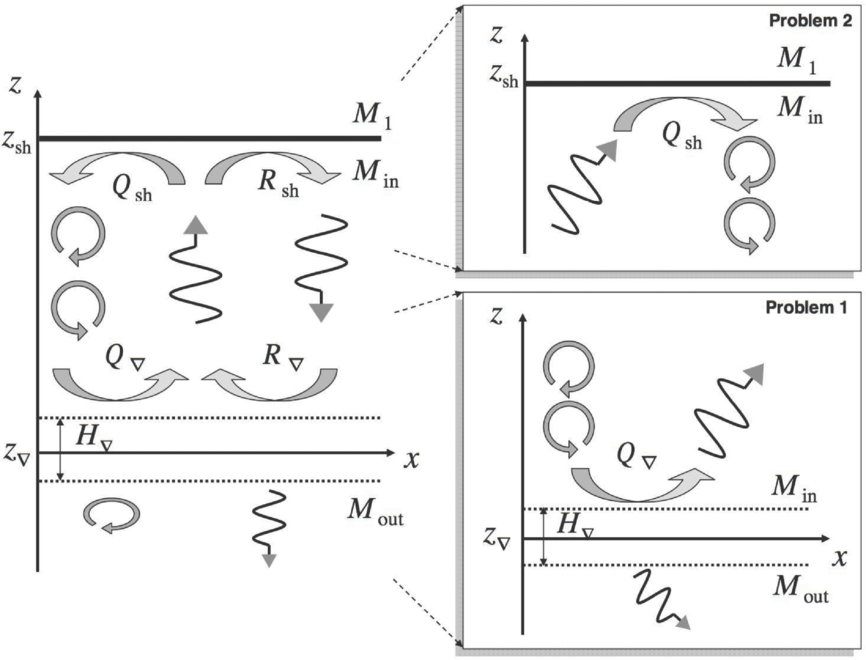
\includegraphics[width=13cm]{figures/Sato1}
\caption {A short caption.}
\label{fig:Sato1}
\end{figure}

For ease of simulation, the potential step and stationary shock are computed separately as sub-problems 1 and 2 respectively. This separation greatly simplifies the introduciton of specific advective and acoustic pertubations to appropriate locations in the interior of the domain, making it much easier to see the interactions of these disturbances at the boundaries (the shock and potential step) between the various flow regions.

\subsection{Sub-Problem 1}
\label{subsec:sub_problem_1}

A hyperbolic tangent function is used to provide a smooth step-like external potential field, with the exact function given by
\begin{equation}
\phi(x)=\frac{\Delta \phi}{2}\left[\textrm{tanh}\left(\frac{y-y_{\nabla}}{H_{\nabla}/2}\right)+1\right],\quad x\in[-2,2],
\end{equation}
where the step size $\Delta \phi$ is set based on the ratio of the sound speeds $c_{\textrm{in}}/c_{\textrm{out}}$ in the constant regions surrounding the step.

\subsection{Sub-Problem 2}

Description of the standing shock
\chapter{Conclusion}
\label{chap:conclusion}

In conclusion...

%% Uncomment both lines to add appendix
%\appendix
%\chapter{Dummy Appendix}

You can defer lengthy calculations that would otherwise only interrupt
the flow of your thesis to an appendix.


\backmatter

\bibliographystyle{unsrt}
\bibliography{refs}

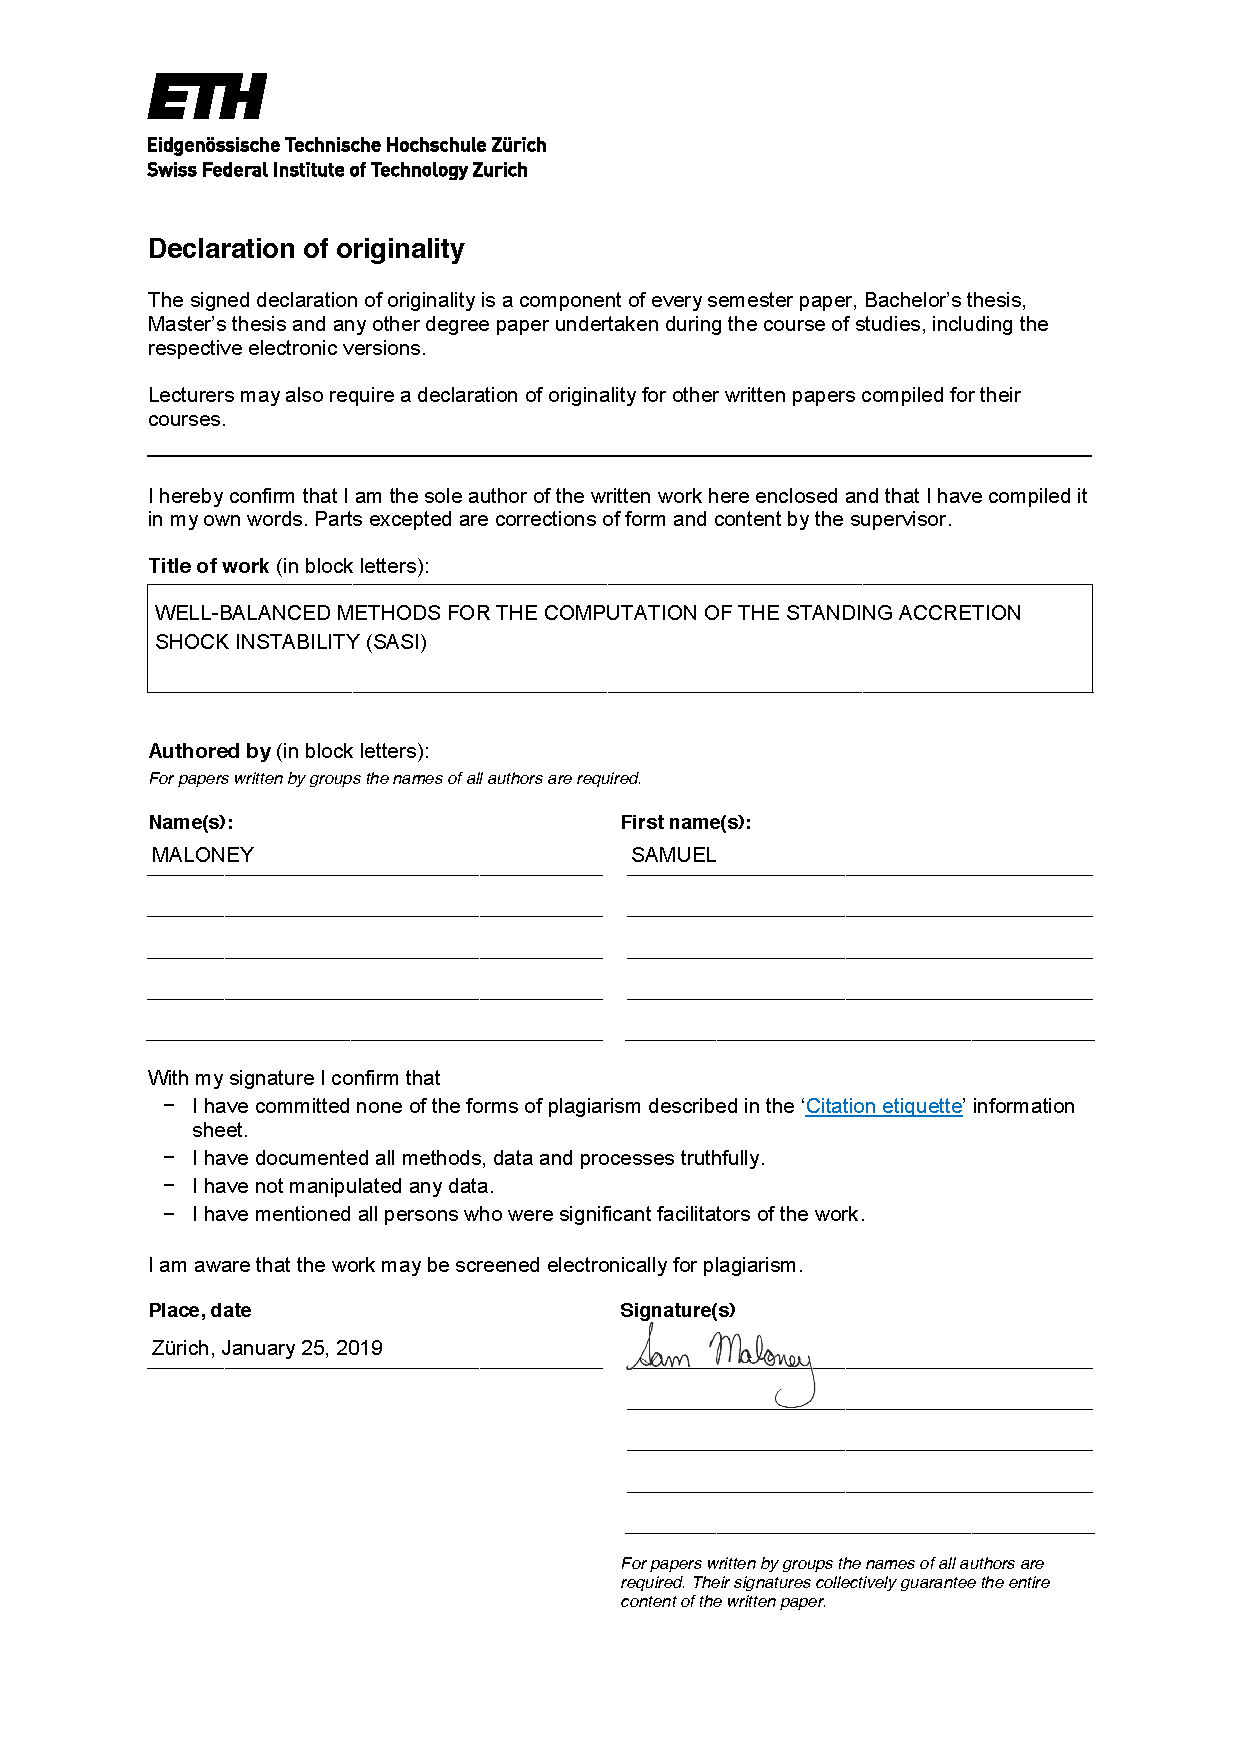
\includepdf[pages={-}]{declaration-originality.pdf}

\end{document}
